% Created 2022-12-01 Thu 19:18
% Intended LaTeX compiler: pdflatex
\documentclass[11pt,a4paper]{article}
    \usepackage[utf8]{inputenc}
    \usepackage[T1]{fontenc}
    \usepackage{fixltx2e}
    \usepackage{graphicx}
    \usepackage{longtable}
    \usepackage{float}
    \usepackage{wrapfig}
    \usepackage{rotating}
    \usepackage[normalem]{ulem}
    \usepackage{amsmath}
    \usepackage{textcomp}
    \usepackage{marvosym}
    \usepackage{wasysym}
    \usepackage{amssymb}
    \usepackage{hyperref}
    \usepackage{mathpazo}
    \usepackage{color}
    \usepackage{enumerate}
    \definecolor{bg}{rgb}{0.95,0.95,0.95}
    \tolerance=1000
                    \usepackage{listings}
\usepackage{xcolor}
\lstset{language=Python,backgroundcolor=\color{black!5}, basicstyle=\footnotesize\ttfamily, columns=fullflexible, breaklines, frame= tb}

    \linespread{1.1}
    \hypersetup{pdfborder=0 0 0}
\author{Ved Patel 67 Vijay Panchal 68}
\date{\today}
\title{Approximations in physics}
\hypersetup{
 pdfauthor={Ved Patel 67 Vijay Panchal 68},
 pdftitle={Approximations in physics},
 pdfkeywords={},
 pdfsubject={},
 pdfcreator={Emacs 28.1 (Org mode 9.5.2)}, 
 pdflang={English}}
\begin{document}

\maketitle
\tableofcontents

\pagebreak
\section{Introduction}
\label{sec:org252628d}

Approximation method is yet most essential topic in physics. Also, approximation is yet essential trick for physicists. Physicists love to do approximations, like in functional expansion for getting polynomials for their ease or may be specialized idealization in particular topic. Approximation help them to \textbf{seeing through physics} instead of going in to maze of exactness in formidable  mathematics. Getting interpretation or i say knowing system is sometime more important then going for regorious mathematics. For example, famous equation of fluid dynamics \textbf{Navier-Stoke equation} can be imposible to solve but as physicist they know what it is.

Be aware, that approximation is just approximation. We should remember everytime we do that. Sometime we forgot actual system which is far from ideal. We should know that we are on mission to know nature not just building new theories.

Let's dive into one example, that showes implication of approximations. In classical mechanics, we have some major theories, one is of oscillatory motions. In Oscillation theory we studied \textbf{Simple Harmonic Oscillation}, but as we are going to see that simple harmonic oscillation is not exactly that simple without approximation. We had actually changed whole system unknowingly, but beauty of physics is that it is still help to understand concept and motion of it. 

\section{Example of Approximation}
\label{sec:org2bb1710}

Approximation is used in almost every branch of physics, not just physics but every field of sciences. We are going to give profound example of understanding advantages and disadvantages of approximation.

\subsection{Defining a problem}
\label{sec:orgb8c40e5}

We learned simple pendulum from very starting of physics course. But what if i say that simple pendulum is not actually simple in sense that approximation hide most of things away from our eyes to see.

Let's take one pendulum,by taking length \(l = 1 m\) string (assuming non deforming) attaching to bob of mass \(m = 0.1 kg\). String attached to rigid wall as shown in figure. Then we give it a initial deviation as \(\theta\) initial \(\theta_{0}\). Initial velocity of system \(v_{0}=0\). We have accelaration of \(g=9.8\) downward.

\begin{figure}[htbp]
\centering
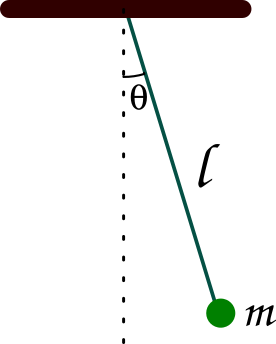
\includegraphics[width=0.3 \textwidth]{./figure1.png}
\caption{\label{fig:orgcb8b6b3}pendulum with string lenth \(l\) and mass \(m\)}
\end{figure}

For understanding consequences of approximation, we took simulations by solving both equation of motion (approximated and exact). For getting equations of motion we used \textbf{Newtonian formulation} which is quite easy to work with in this type of problems, since we are working with \textbf{non conservative} system.


\subsection{Pendulum motion in presence of damping force}
\label{sec:orge2269db}

In real situations we have non-conservative forces affecting on system. In our system we have air resistance acting on bob. This drag force will always be proportional to it's physical shape and size. Since, we can't tell exactly drag force mathematically, We have \textbf{two often used approximations}. Firstly, there is stockes's law of drag which is linearly proportional to the velocity. Then we have Newton's drag law which is quadratically proportional to the velocity.

We will see that how this two approximation affect our system and it's simulation. We also see mathematical forms of this two but firstly, let's define this two damping coefficient.

\subsubsection{Damping by linear to the velocity approximation}
\label{sec:orge02b8e2}

Let's discuss coffiecient of linear damping. Linear to the velocity drag is also called stoke's drag. We can write equation of damping by \(F_{damping} = k_{l}v\). Where, \(k_{l}\) is damping coefficient, value of it depend on shape of object. For our spherical bob it has for of \(k_{l} = 3\pi\eta d\), where \(\eta\) is dynamic viscosity of medium and have values of \(\eta = \rho \nu\). We have \(d\) as diameter of sphere, for our purpose we are using as \(d=0.01m\). 

\subsubsection{Damping by quadratic to the velocity approximation}
\label{sec:org20da46a}

We used quadratic damping approximation as nonlinear damping approximation. This is also called newton's drag and it's better approximation then linear one. As quantitatively it can work with turbulent flow with 1000 to 100000 reynolds number. Where linear approximation works reynold's number upto 1. Quadratic damping is better than linear approximation but we can't have close form solution, it is the reason we use linear damping approximation. In quadratic damping it has following form, \(F_{damping} = k_{q} v^{2}\). Here, \(k_{q} = \frac{1}{8}c_{d}\rho \pi d^{2}\), where \(c_{d}\) is drag coefficient and has value of 0.47. \(\rho\) and \(d\) are density of fluid and diameter.\cite{lubarda2021analysis}\cite{goossens2019review}


\subsection{General equation motion}
\label{sec:org9a3bc1f}

Let's derive equation of motion for our system which can be modified as we took approximations in it. We have Figure 1 showing pendulum with unextensible string of length \(l\) with sphere of diameter \(d\) and mass \(m\). Our system is in fluid with density \(\rho\) and viscosity \(\eta\). Let's use newton's law of motion to derive equation of motion,

First of all, we compared horizontal and vertical forces.

\begin{equation}
\label{eq:org95b22bb}
   F_{damping}cos(\theta)-Tsin(\theta)=ma_{x}
\end{equation}
\begin{equation}
\label{eq:orge2d587c}
   F_{damping}sin(\theta)+Tcos(\theta)-mg=ma_{y}
\end{equation}

Adding equation \ref{eq:org95b22bb} and equation \ref{eq:orge2d587c} with multiplication by \(cos(\theta)\) and \(sin(\theta)\) respectively.

\begin{equation*}
\label{eq:org68cab11}
F_{damping}sin^{2}(\theta)+F_{damping}cos^{2}(\theta)-mgsin(\theta)=ma_{x}cos(\theta)+ma_{y}sin(\theta)
\end{equation*}

\begin{equation*}
\label{eq:org945e099}
F_{damping}-mgsin(\theta)=m(asin^{2}(\theta)+acos^{2}(\theta))
\end{equation*}

\begin{equation}
\label{eq:org10da393}
F_{damping}-mgsin(\theta)=ma
\end{equation}

From,
\begin{equation*}
\label{eq:org9e43cbb}
a = (\ddot{r}-r\dot{\theta}^{2})\hat{r} + (r \ddot{\theta}+2\dot{r}\dot{\theta})\hat{\theta}
\end{equation*}

Where,  \(r=l\) and since \(\dot{l}=0\), \(a=l\ddot{\theta}\). So, equation \ref{eq:org10da393} becomes,

\begin{equation}
\label{eq:orgee934b2}
F_{damping}-mgsin(\theta)=ml\ddot{\theta}
\end{equation}

This is \textbf{exact equation of motion}. Which will be \textbf{second order non linear equation}. Finding it's exact solution is another ordeal. Let's take our approximations and cases for it.

\subsection{Approximation of equation of motion : Linear differential equation with linear damping}
\label{sec:org6a81754}

In class, we approximated equation \ref{eq:orgee934b2} as \(\theta \to 0\) as \(sin(\theta) \to \theta\). Consequently, this equation becomes very easy to solve. Also, damping force will be,

\begin{equation*}
\label{eq:org1edbe4c}
F_{damping}=-k_{l}v
\end{equation*}

\begin{equation*}
\label{eq:org57d88bc}
F_{damping}=-k_{l}l\dot{\theta}
\end{equation*}

So, equation \ref{eq:orgee934b2} becomes,

\begin{equation}
\label{eq:org787b214}
\ddot{\theta}+\frac{k_{l}l}{m}\dot{\theta}+\frac{g}{l}\theta=0
\end{equation}

\begin{equation}
\label{eq:org3fc0b31}
\ddot{\theta}+\Gamma\dot{\theta}+w_{0}^{2}\theta=0
\end{equation}

Where, we took \(\Gamma = \frac{k_{l}l}{m}\) and \(w_{0}^{2}\).

We can solve this linear equation \ref{eq:org3fc0b31} by usual methods of linear differential equation. Simply taking \(\theta=e^{\lambda t}\), which gives polynomials of second order.

\begin{equation}
\label{eq:org0d3fbd3}
\lambda^{2}+\Gamma\lambda+w_{0}^{2}=0
\end{equation}

We can find roots of this quadratic equation.

\begin{equation}
\label{eq:orgf26ae96}
\lambda = \frac{-\Gamma}{2} \pm \frac{\sqrt{\Gamma^{2}-4w_{0}^{2}}}{2}
\end{equation}

\begin{equation}
\label{eq:org08026ea}
\lambda = \frac{-\Gamma}{2} \pm \sqrt{\frac{\Gamma}{2}^{2}-w_{0}^{2}}
\end{equation}

Here we getting three type of roots,

\begin{enumerate}
\item Roots where \(\frac{\Gamma}{2}=w\). this is \textbf{critical damping condition}, where we getting \(\lambda=\frac{-\Gamma}{2}\). Putting \(\lambda\) into our solutions, \(\theta = e^{\frac{-\Gamma}{2}t}\). Which suggest this will only decay with time and never overshoots from equilibrium position. Which is desired in certain condition but not for us.

\item Roots where \(\frac{\Gamma}{2}>w\). this is \textbf{overdamping condition}, where we getting \(\lambda=\frac{-\Gamma}{2}\pm\sqrt{\frac{\Gamma}{2}^{2}-w_{0}^{2}}\). So from here we get \(\theta = e^{\frac{-\Gamma}{2}t}e^{\pm\sqrt{\frac{\Gamma}{2}^{2}-w_{0}^{2}}t}\). This also have exponential term in it which will only decay with time and never overshoots from equilibrium position.

\item Roots where \(\frac{\Gamma}{2}<w\). this is \textbf{underdamping condition}, here  \(\lambda=\frac{-\Gamma}{2}\pm i\sqrt{w_{0}^{2}-\frac{\Gamma}{2}^{2}}\). \(\theta = e^{\frac{-\Gamma}{2}t}e^{\pm i \sqrt{w_{0}^{2}-\frac{\Gamma}{2}^{2}}t}\). This has complex term, which implicitly suggest that it'll overshoot and oscillate. This our topic of interest for this project.
\end{enumerate}


Without forgetting our initial system we came to we took third case as our solution.

\begin{equation*}
\label{eq:org1eea347}
\Therefore \theta = e^{\frac{-\Gamma}{2}t}e^{\pm i \sqrt{w_{0}^{2}-\frac{\Gamma}{2}^{2}}t}
\end{equation*}

Taking \(w^{2} = w_{0}^{2}-\frac{\Gamma}{2}^{2}\). And writing our solution in linear combination from above equation,

\begin{equation}
\label{eq:org93684be}
\theta = e^{\frac{-\Gamma}{2}t}(C_{1}e^{iwt}+C_{2}e^{-iwt})
\end{equation}

Taking real part of equation \ref{eq:org93684be}. Since it'll represent real motion of system. At last we get equation like this,

\begin{equation}
\label{eq:org51fa811}
\theta = e^{\frac{-\Gamma}{2}t}A cos(wt-\delta)
\end{equation}

Where, \(A\) and \(\delta\) can be find from initial conditions and \(w = \sqrt{w_{0}^{2}-\frac{\Gamma}{2}^{2}}\).

\subsection{Non linear equation of motion with linear damping}
\label{sec:org8675830}

In equation \ref{eq:orgee934b2} we can write linear damping term without taking approximation as \(sin(\theta) \to \theta\),

Writing again \ref{eq:orgee934b2}, 
\begin{equation*}
\label{eq:org67d53c2}
F_{damping}-mgsin(\theta)=ml\ddot{\theta}
\end{equation*}

Here, putting \(F_{damping}=-k_{l}l\dot{\theta}\) will give us,

\begin{equation}
\label{eq:orgabe5879}
\ddot{\theta}+\frac{k_{l}l}{m}\dot{\theta}+\frac{g}{l}sin(\theta)=0
\end{equation}

This is second order nonlinear equation we can't get it's closed form solution but we can get numerical one. Let's make it easy to use in numerical methods.

Take \(\phi = \dot{\theta}\) and \$\frac\{k\textsubscript{l}l\}\{m\}=\(\Gamma\)\$so, equation \ref{eq:orgabe5879} becomes,

\begin{equation}
\label{eq:org2e4247b}
\dot{\phi}+\Gamma\phi=-\frac{g}{l} sin(\theta)
\end{equation}

We can use numerical methods like Runge-Kutta method to solve this equation. I have given brief overview of runge kutta methods in appendix 1. For that we define \(\phi\) and \(\dot{\phi}\) as following,

\begin{equation}
\label{eq:orge3cf3da}
\phi=\dot{\theta}
\end{equation}

\begin{equation}
\label{eq:org6039144}
\dot{\phi}=-\Gamma\phi-\frac{g}{l} sin(\theta)
\end{equation}

We have two complementary equations \ref{eq:orge3cf3da} and \ref{eq:org6039144}. We can use now Runge-Kutta method on it. I have used in my code file \emph{main.py}, you can access it in appendix. 

\subsection{Simulations of the two equations}
\label{sec:orga364d7b}

I have done nice simulation which give hands on experience of two equation, both have very similar results when \(\theta\) is very small, again understandable as \(\theta \to 0\) we can approximate \(sin(\theta) \to \theta\). But when \(\theta\) increase slightly we have massive changes in solution with time. Let's look at \(\theta = \frac{\pi}{10}\), (here, we take viscosity of air at \((1834·38\pm0.35)\times10^{−7}\) c.g.s. units. \cite{majumdar1938coefficient})

Initially both are same as you can see in pictures (at \(t=0\)),
\begin{figure}[htbp]
\centering
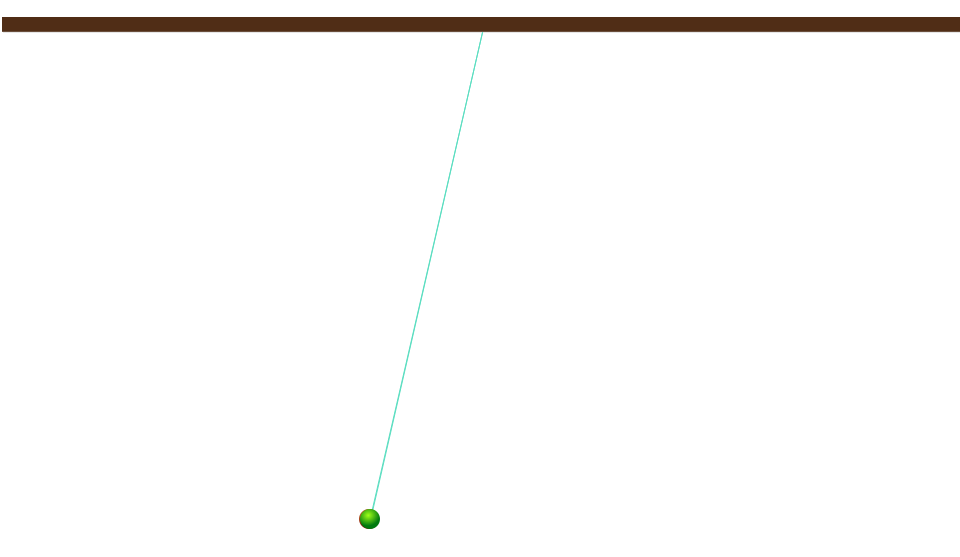
\includegraphics[width=0.8 \textwidth]{t0.png}
\caption{\label{fig:orgd6fedb6}pendulum at \(t=0s\)}
\end{figure}

Now, as we look with increment in time we can see it deflecting slightly with it. This is picture at \(t = 100s\),
\begin{figure}[htbp]
\centering
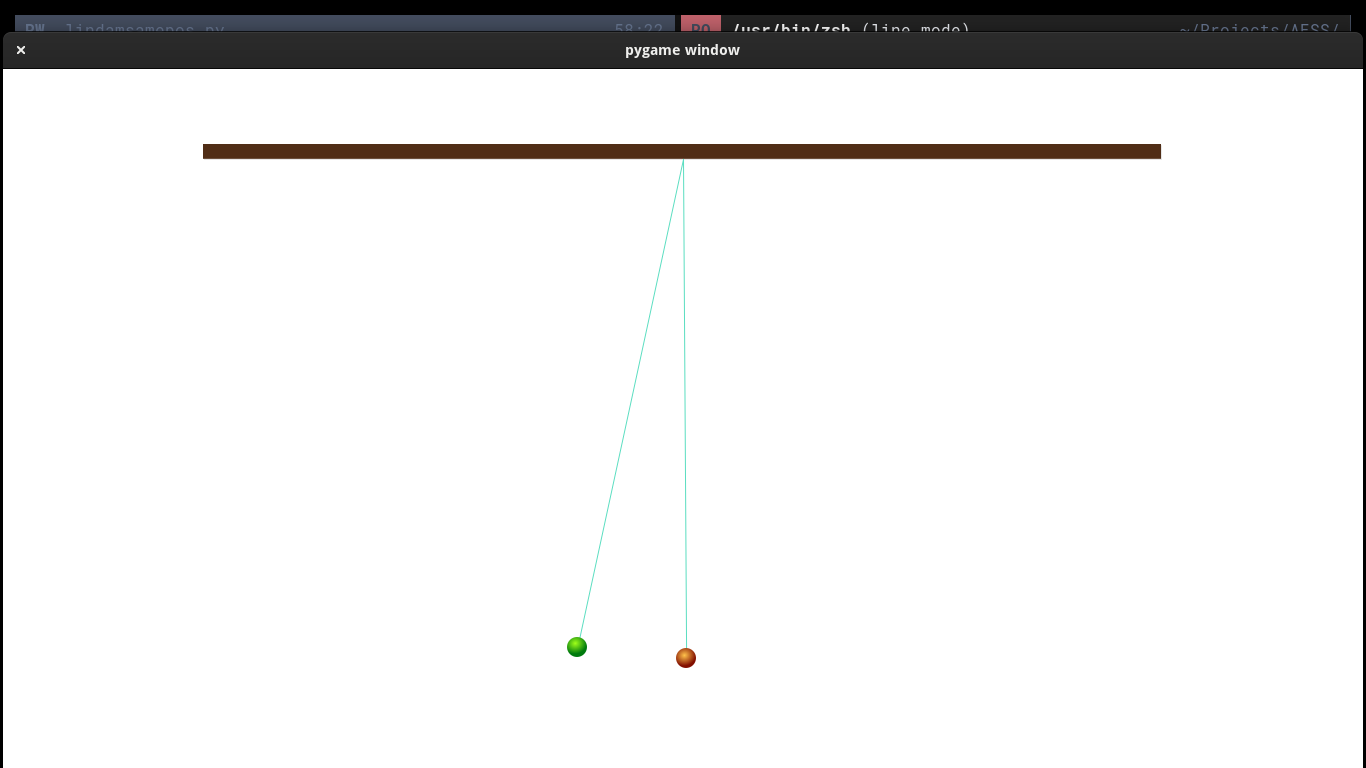
\includegraphics[width=0.8 \textwidth]{t100.png}
\caption{\label{fig:org13c368e}pendulum at \(t=100s\)}
\end{figure}

Here, red bob is exact solution (nonlinear equation) where green is linear equations solution.

For more information, i gave all my code in appendix and also in my github page \href{https://github.com/vijaypanchalr3}{vijaypanchalr3}.

\subsection{Equation of motion with quadratic damping}
\label{sec:org0a4eb34}

Quadratic damping gives better approximations over as linear damping but also gives burden of nonlinearization. 


\section{Results and conclusion}
\label{sec:org893982d}

As we seen earlier our simulations discuss how exact solution differs from approximation. Also, we see that linear damping is still a approximation and can be replaced by better approximation when medium have turbulant flow by bob of our pendulum.

\subsection{Effect on angular frequency of pendulum with approximation and exact solution}
\label{sec:orgb8bb19b}

As we have seen in our simulation that in linear solution equation \ref{eq:org51fa811}, we got single constant frequency with \(\theta\) but not in nonlinear one. Nonlinear equation has non constant frequency. We can see from graph of it that how it differs from constant frequency of linear solution.

\begin{figure}[htbp]
\centering
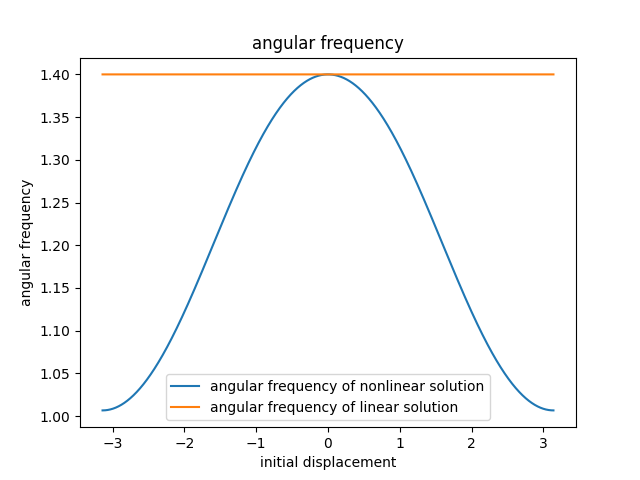
\includegraphics[width=0.8 \textwidth]{angfre.png}
\caption{\label{fig:org259381a}figure 4   how angular frequency change with \(\theta_{0}\) in nonlinear solution and shows constant at value \(\sqrt{\frac{g}{l}}\)}
\end{figure}


\subsection{For different \(\theta_{0}\) it has different \(\theta(t)\)}
\label{sec:org673677e}

Let's look at how our two solution exactly changes with time. For that we took values of \(\theta\) on time scale and changed it's \(\theta_{0}\).





\subsection{Hidden informations}
\label{sec:orge1fdb9f}

Approximation not only affect in quantitatively but also sometimes qualitatively. Let's discuss part of that lost in approximation. Phase planes are geometrical procedures of obtaining properties of system (here solutions). If write our equation of motion for the pendulum from \ref{eq:orgee934b2}.

\begin{equation*}
\label{eq:org106de76}
F_{damping}-mgsin(\theta)=ml\ddot{\theta}
\end{equation*}

Here, \(F_{damping}\) is velocity depend term. Also, velocity \(v=l\dot{\theta}\). So, we can write equation \ref{eq:orgee934b2} in following way,


\begin{equation*}
\label{eq:orgfc94e10}
F_{d}(\dot{\theta})-mgsin(\theta)=ml\ddot{\theta}
\end{equation*}

Taking \(\phi=\dot{\theta}\) led to,

\begin{equation}
\label{eq:org235eb10}
\dot{\phi}=(\frac{1}{ml})F_{d}(\phi)-\frac{g}{l}sin(\theta)
\end{equation}

\begin{equation}
\label{eq:org7483746}
\dot{\theta} = P(\theta,\phi)
\end{equation}

\begin{equation}
\label{eq:org5c265f5}
\dot{\phi} = Q(\theta,\phi)
\end{equation}

Dividinge equation \ref{eq:org5c265f5} and \ref{eq:org7483746} will give us,

\begin{equation}
\label{eq:org30b86c4}
\frac{\dot{\phi}}{\dot{\theta}}= \frac{\frac{d(\phi)}{dt}}{\frac{d{\theta}}{dt}} = \frac{d\phi}{d\theta}= \frac{Q(\theta,\phi)}{P(\theta,\phi)}
\end{equation}

This equation \ref{eq:org30b86c4} will give \textbf{phase trajectory} of our system. By, equation \ref{eq:org235eb10} value of \(\phi\) gives,

\begin{equation}
\label{eq:org3977e72}
\frac{d\phi}{d\theta}=\frac{(\frac{1}{ml})F_{d}(\phi)-\frac{g}{l}sin(\theta)}{phi}
\end{equation}

In equation \ref{eq:org3977e72} if we put value of \(F_{d} = k_{l}l\dot{\theta} = k_{l}l\phi\) for linear damping damping force, we will get,

\begin{equation}
\label{eq:orgf0d9fc2}
\frac{d\phi}{d\theta}=\frac{\Gamma\phi-\frac{g}{l}sin(\theta)}{phi}
\end{equation}

This is our equation of motion which give trajectory for exact solution and similarly approximated solution would be,

\begin{equation}
\label{eq:orgb4885f9}
\frac{d\phi}{d\theta}=\frac{\Gamma\phi-\frac{g}{l}\theta}{phi}
\end{equation}

Ploting this two will give two distinct phase planes which gives important properties of system. Two phase plane plots are as following, 


\begin{figure}[htbp]
\centering
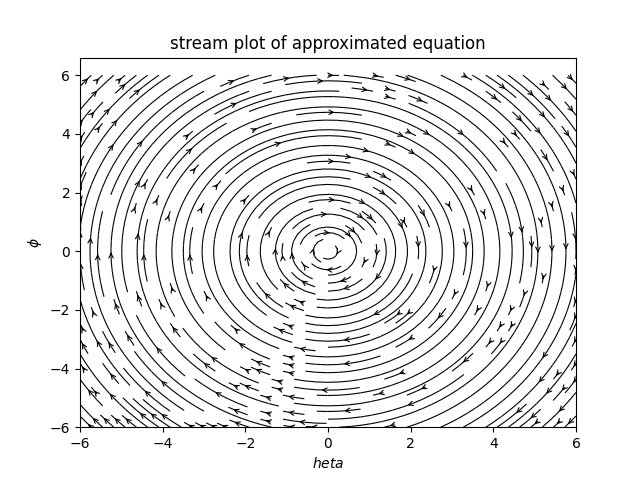
\includegraphics[width=0.8 \textwidth]{approlstr.png}
\caption{\label{fig:orgabb9853}figure 5 this is phase plane of approximate solution where we took \(sin(\theta) \to \theta\). here you can see big vortex.}
\end{figure}

\begin{figure}[htbp]
\centering
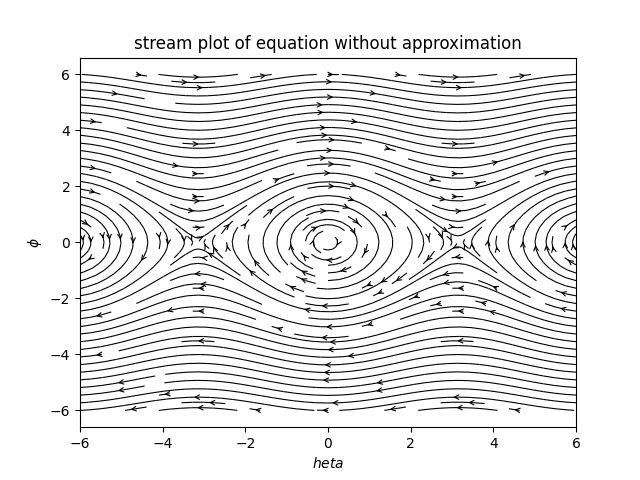
\includegraphics[width=0.8 \textwidth]{exactlstr.png}
\caption{\label{fig:orgdf3a90a}figure 6 this is phase plane of exact solution without previous approximation.}
\end{figure}

As we can see that in approximated equation we have only one big vortex. In contrast to that we have vortexs with lines.

In first figure in approximated equation we have phase trajectory of simplest, spiral. This suggest a simple harmonic motion which will always have stable and periodic motion.

In second figure we got completely different phase trajectory. We got three are with completely different behavior of system. The three cases of it are following,

In first area, which is vortex like previous has stable and periodic with energy \(E<2mgl\), second area we got \textbf{seddle point}, in which we got unstable and aperiodic motion (\(E=2mgl\)). In last area which is upper and lower part of plot are just lines, this are shows circular motion around pivot of string with wall. Energy for this kind of motion is \(E>2mgl\).











\break

\section{Appendix}
\label{sec:org9b97c85}
\subsubsection{(Appendix:1) Understand Runge-Kutta method}
\label{sec:org97a202d}

In our this simulation we made use of Range Kutta fourth order method as numerical method for solving non-linear differential equation and linear differential equation with it. So, it is good idea to understand what is Range-Kutta fourth order method and how can we implement to solve present differential equations.

Runge Kutta Method is not predictor-corrector method like other numerical method (namely, modified Euler method, Adams-Bashmoth-Moulton method) for solving differential equation. It uses four different new variables and then simply addition and multiplication predict our initial value problem with good accuracy.

We can use RK method in following manor,

\begin{equation*}
y_{n+1} = y_{n}+\frac{1}{6}(k_{1}+2k_{2}+2k_{3}+k_{4})
\end{equation*}

\begin{equation*}
z_{n+1} = z_{n}+\frac{1}{6}(l_{1}+2l_{2}+2l_{3}+l_{4})
\end{equation*}

Where,
\begin{equation*}
k_{1}=hf(x_{n},y_{n},z_{n})
\end{equation*}
\begin{equation*}
l_{1}=hg(x_{n},y_{n},z_{n})
\end{equation*}
\begin{equation*}
k_{2}=hf(x_{n}+\frac{h}{2},y_{n}+\frac{k_{1}}{2},z_{n}+\frac{l_{1}}{2})
\end{equation*}
\begin{equation*}
l_{2}=hg(x_{n}+\frac{h}{2},y_{n}+\frac{k_{1}}{2},z_{n}+\frac{l_{1}}{2})
\end{equation*}
\begin{equation*}
k_{3}=hf(x_{n}+\frac{h}{2},y_{n}+\frac{k_{2}}{2},z_{n}+\frac{l_{2}}{2})
\end{equation*}
\begin{equation*}
l_{3}=hg(x_{n}+\frac{h}{2},y_{n}+\frac{k_{2}}{2},z_{n}+\frac{l_{2}}{2})
\end{equation*}
\begin{equation*}
k_{4}=hf(x_{n}+h,y_{n}+k_{3},z_{n}+l_{2})
\end{equation*}
\begin{equation*}
l_{4}=hg(x_{n}+h,y_{n}+k_{3},z_{n}+l_{2})
\end{equation*}

Where, \(h\) is step and \(f,g\) are two complimetry function, in our purpose we used \(f = \theta\) and \(f = \phi\).





\subsubsection{Simulation code}
\label{sec:orga63b9eb}

Now, come animation part. Which we basically used \textbf{pygame} in \textbf{python}. We first get array of both solutions with interval of \(\frac{1}{60} second\) and give this data in position function in my \emph{main.py} file which just use convert each to the Cartesian coordinates from initial Polar coordinate. This is because \emph{pygame} screen rectangular coordinates with units in pixel of screen.

Following data, we used as constant which i defined in \emph{constant.py} file, as per close inspection you can see that we used C.G.S. units because of better visual on computer screen. Remember, we made this code for reconstruct purpose only.

My \emph{constant.py} file

\begin{lstlisting}language=Python]
  from math import sqrt

  # defining constants in C.G.S.

  pi = 3.141592
  width,height = 1360,720         # pygame window size in pixel units
  origin_x,origin_y = width/2,height/8 # setting up the origin O

  # density
  rho = 0.001293

  # newton's drag coefficient
  cd = 0.47

  # diameter
  d = 0.05

  # mass 
  m = 500

  # length of string
  l = 500

  # gravitation accelaration
  g = 980

  # viscosity of air
  eta = 0.0001834

  kl = 3*pi*eta*d
  kq = (1/8)*pi*cd*rho*d*d

  gammal = (kl*l)/m
  gammaq = (kq*l)/m
  w0 = sqrt(g/l)                  # natural frequncy of SHM
  theta_initial = 3.141592/10      # initial theta in radian
  radius = 10                     # radius of ball in pixel
  fps = 120                        # frame per second



\end{lstlisting}

This is my \emph{main.py} file, in which i defined all functions for calculations. In which, i have Runge-Kutta method defined and solution and also phase planes defined.

\begin{lstlisting}[language=Python]

  from constants import *
  from numpy import sin, sqrt, zeros

  def f2nonlinear_linear(theta,phi):     # we defined second auxillary equation from nonlinear term.
      return -((gammal)*phi)-(w0*sin(theta))

  def f2linear_linear(theta,phi):        # we defined second auxillary equation from linear term.
      return -((gammaq)*phi)-(w0*theta)

  def f2llinear_nonlinear(theta,phi):        # we defined second auxillary equation from linear term.
      return -((kq)*phi*phi)-(w0*theta)

  def f2nonlinear_nonlinear(theta,phi):        # we defined second auxillary equation from linear term.
      return -((kq)*phi*phi)-(w0*sin(theta))



  # range-kutta method defined
  def RK4(theta,phi,h,K): 
      h = h/8
      for i in range(8):
          k1 = h*phi
          l1 = h*K(theta,phi)
          k2 = h*(phi+(l1*0.5))
          l2 = h*(K(theta+(k1*0.5),phi+(l1*0.5)))
          k3 = h*(phi+(l2*0.5))
          l3 = h*(K(theta+(k2*0.5),phi+(l2*0.5)))
          k4 = h*(phi+l3)
          l4 = h*(K(theta+k3,phi+l3))
          k_ = (1/6)*(k1+k4+2*(k2+k3))
          l_ = (1/6)*(l1+l4+2*(l2+l3))
          theta+=k_
          phi+=l_
      return theta,phi

  # Solutions of linear term ---- gives array of length (Total_time*fps)
  def linear_linear(theta_initial,Total_time,fps):
      linear_solutions = zeros([Total_time*fps+2])
      linear_solutions[0] = theta_initial
      phi = zeros([Total_time*fps+2])
      phi[0],t = 0,0
      while t<Total_time*fps:
          linear_solutions[t+1], phi[t+1] = RK4(linear_solutions[t],phi[t],1/fps,f2linear_linear)
          t+=1
      return linear_solutions

  def linear_nonlinear(theta_initial,Total_time,fps):
      linear_solutions = zeros([Total_time*fps+2])
      linear_solutions[0] = theta_initial
      phi = zeros([Total_time*fps+2])
      phi[0],t = 0,0
      while t<Total_time*fps:
          linear_solutions[t+1], phi[t+1] = RK4(linear_solutions[t],phi[t],1/fps,f2llinear_nonlinear)
          t+=1
      return linear_solutions

  # Solutions of nonlinear term ---- gives array of length (Total_time*fps)
  def nonlinear_linear(theta_initial,Total_time,fps):
      nonlinear_solutions = zeros([Total_time*fps+2])
      nonlinear_solutions[0] = theta_initial
      phi = zeros([Total_time*fps+2])
      phi[0],t= 0,0
      while t<Total_time*fps:
          nonlinear_solutions[t+1], phi[t+1] = RK4(nonlinear_solutions[t],phi[t],1/fps,f2nonlinear_linear)
          t+=1
      return nonlinear_solutions

  def nonlinear_nonlinear(theta_initial,Total_time,fps):
      nonlinear_solutions = zeros([Total_time*fps+2])
      nonlinear_solutions[0] = theta_initial
      phi = zeros([Total_time*fps+2])
      phi[0],t= 0,0
      while t<Total_time*fps:
      nonlinear_solutions[t+1], phi[t+1] =     RK4(nonlinear_solutions[t],phi[t],1/fps,f2nonlinear_nonlinear)
      t+=1
      return nonlinear_solutions

  # ------------(for graphs)----------
  # this describes frequncy of nonlinear term.
  def w_nonliner(theta_initial):
  w_ =     (sqrt(l/g))*(1+(0.25*(sin(0.5*theta_initial))**2)+((9/64)*(sin(theta_initial*0.5))**4))
  return 1/w_

  # phase plane definations
  def linear_phase_plane(theta,phi):
      f1 = phi
      f2 = -((gammal)*phi)-(w0*theta)
      return f1,f2

  def nonlinear_phase_plane(theta,phi):
      f1 = phi
      f2 = -((gammal)*phi)-(w0*sin(theta))
      return f1,f2

  def linear_phase_planeq(theta,phi):
      f1 = phi
      f2 = -((gammaq)*phi*phi)-(w0*theta)
      return f1,f2

  def nonlinear_phase_planeq(theta,phi):
      f1 = phi
      f2 = -((gammaq)*phi*phi)-(w0*sin(theta))
      return f1,f2



  # ----------------------------------

\end{lstlisting}

Simulation files are \emph{lindamsamepos.py}, \emph{nonlindamsamepos.py} and also two other \emph{lindamdiffpos.py} and \emph{nonlindamdiffpos.py}. In the files respecevely i put my code for linear damping with same pivot position and also quadratic damping with same position of pivot. Other two files are complementary for different pivot position not much of importance.

I am writing here my linear damping file for regeneration perpose in other two i just changed fuction name from \emph{main.py}.

\begin{lstlisting}[language=Python]

  from main import *
  import pygame
  import time
  from numpy import cos, sin, pi


  # this part done.
  # just do - [ ] dual color balls



  def bob1(window,x,y):
      image = pygame.image.load("bitmap1.png")
      window.blit(image, (x,y))

  def bob2(window,x,y):
      image = pygame.image.load("bitmap2.png")
      window.blit(image, (x,y))

  def surface(window,x,y):
     image = pygame.image.load("surface.png")
     window.blit(image, (x, y))



  def position(l,theta):
     return origin_x-10+l*cos((1.5*pi)-theta),origin_y-10-l*sin((1.5*pi)-theta)

  def mainloop(window,fps):
      global t
      run = True
      clock = pygame.time.Clock()
      c = 0
      while run:
          for event in pygame.event.get():
              if event.type== pygame.QUIT:
                  run= False
                  break
          clock.tick(fps)

          x,y = position(l,exact[c])
          x2,y2 = position(l,appro[c])
          if c==len(exact):
              break
          window.fill("#ffffff")
          surface(window,200,origin_y-15)
          pygame.draw.aaline(window,color="#5BDEC1",start_pos=(origin_x,origin_y),end_pos=(x+radius,y+radius))
          pygame.draw.aaline(window,color="#5BDEC1",start_pos=(origin_x,origin_y),end_pos=(x2+10,y2+10))
          bob1(window,x,y)
          bob2(window,x2,y2)
          pygame.display.update()
          c+=1
          pygame.quit()

  if __name__ == "__main__":
      pygame.init()
      window = pygame.display.set_mode((width,height))
      exact = nonlinear_linear(theta_initial,300,fps)
      appro = linear_linear(theta_initial,300,fps)
      t = time.perf_counter()
      mainloop(window, fps)


\end{lstlisting}

\subsubsection{Code for graphs}
\label{sec:org6aba5fa}

This is code for all the graphs in pdf.
\begin{lstlisting}[language=Python]
    from main import *
import numpy as np
import matplotlib.pyplot as plt




def angfre():
    A = np.linspace(-np.pi,np.pi,6000)
    w = np.zeros(np.size(A))
    w0 = np.zeros(np.size(A))

    for i in range(np.size(A)):
        w[i] = w_nonliner(A[i])
        w0[i] = np.sqrt(g/l)

    
    plt.figure()
    plt.plot(A,w, label="angular frequency of nonlinear solution")
    plt.plot(A,w0, label="angular frequency of linear solution")
    plt.title("angular frequency")
    plt.ylabel("angular frequency")
    plt.xlabel("initial displacement")
    plt.legend()
    plt.savefig("angfre.png")
    plt.close
    
def thetawitht(total_time):
    fig, axes = plt.subplots(2, 2, sharex=True, sharey=True)
    # add a big axes, hide frame
    fig.add_subplot(111, frameon=False)
    
    # hide tick and tick label of the big axes
    plt.tick_params(labelcolor='none', top=False, bottom=False, left=False, right=False)
    # plt.grid(False)
    plt.xlabel("time")
    plt.ylabel("angular displacement")
    plt.title("angualar displacement with time")
    time  = np.linspace(0,total_time,1002)

    # fig.add_subplot(411,frameon=False)
    # ax1 = plt.subplot(111)
    plt.tick_params(labelcolor='none', top=False, bottom=False, left=False, right=False)
    theta_initial = pi/10
    soll = linear_linear(theta_initial,total_time,int(1000/total_time))
    soln = nonlinear_linear(theta_initial,total_time,int(1000/total_time))
    plt.plot(time,soll)
    
    plt.show()

  \end{lstlisting}

And this code for phase plane plots,
\begin{lstlisting}[language=Python]
    from numpy import linspace, meshgrid
from main import *
import matplotlib.pyplot as plt


def exact_lineardamp():
    x1 = linspace(-6,6,2000)
    x2 = linspace(-6,6,2000)

    x1_,x2_ = meshgrid(x1,x2)

    u,v = nonlinear_phase_plane(x1_,x2_)
    vel = sqrt(u**2+v**2)

    plt.figure()
    plt.streamplot(x1_,x2_,u,v, color='k', linewidth=0.8,density=1.5, minlength=0.01, arrowsize=0.8,arrowstyle="->")
    plt.title("stream plot of equation without approximation")
    plt.xlabel("$\theta$")
    plt.ylabel("$\phi$")
    plt.savefig("exactlstr.png")

def appro_lineardamp():
    x1 = linspace(-6,6,2000)
    x2 = linspace(-6,6,2000)

    x1_,x2_ = meshgrid(x1,x2)

    u,v = linear_phase_plane(x1_,x2_)
    vel = sqrt(u**2+v**2)

    plt.figure()
    plt.streamplot(x1_,x2_,u,v, color='k', linewidth=0.8,density=1.5, minlength=0.01, arrowsize=0.8,arrowstyle="->")
    plt.title("stream plot of approximated equation")
    plt.xlabel("$\theta$")
    plt.ylabel("$\phi$")
    plt.savefig("approlstr.png")

exact_lineardamp()
appro_lineardamp()

  \end{lstlisting}




\addcontentsline{toc}{section}{References}
\bibliographystyle{plain}
\bibliography{documentaion}
\end{document}